\chapter{Custom Implementation}

\section{Program Structure}
\label{structure}

Our goal was to develop a fast \aspop{} solver that would adhere as closely as possible to the literature described in Section \ref{background}, along with the extensions described in Section \ref{extensions}. For the purpose, our system was implemented in the Rust\footnote{Available at \url{https://www.rust-lang.org/en-US/}} programming language, chosen mostly for it's thread-safety and the systems-language speed it provides \cite{rustlang}.

The implementation was structured around an isolated \textit{mode} module that would act as an interface for altering the behavior of the \glspl{filtering scheme} and \glspl{partitioning scheme} for testing; The mode component would define functions to determine:
\begin{enumerate}
\item Pattern partition sizes
\item Filtering scheme
\item Candidate generation condition
\end{enumerate}

Depending on the definition of these functions, the program would implement the schemes of \vali{} and Kucherov, along with any experimental schemes of our own. The idea was to make the program’s behavior as consistent as possible between different modes such that they could be compared and benchmarked experimentally. Additionally, this modular approach allowed for faster iteration on testing of new schemes.
 
The pseudo code in Figure \ref{fig:pseudocode} gives a high-level overview of the program’s processes, which abstracts over the two steps of the algorithm for a single pattern string from the $S$ set as a task. The effects of the mode component are limited to the \gls{search step} of each \gls{task}.

\begin{figure}[!htb]
\centering
\myPython{data/pseudocode.py}
\caption[Python pseudo code for the implementation of the \aspop{} solver.]{Python pseudo code for the implementation of the \aspop{} solver, with details such as multi-threading omitted for brevity.}
\label{fig:pseudocode}
\end{figure}












\section{Additions to the Literature}

\subsection{Resolving Opposing Search Directions} \label{own_impl_search_dir}

The \aspop{} implementation makes use of a conventional \textit{FM-Index} \gls{text index} (See \ref{fmindex}). Due to the nature of the underlying \textsc{bwt} (See \ref{bwt} for more details), the text index is ultimately only capable of matching symbols when searched from \textit{right} to \textit{left}. The existing literature set a precedent of describing the \gls{suffix filter} algorithm \gls{search step} in a forwards direction (from the front to the back of the \gls{pattern}), which results in suffix filters instead of prefix filters.
 
The difference in terminology here (left and right vs. front and back) is deliberate.
 
In this \aspop{} implementation, $S$ strings are indeed searched from front to back, but the front of the strings lie \textit{right} of the back of the strings, in terms of index positions and so forth. \vali{} refer to this as a `simulated forwards search' \cite{vali2010}. This unintuitively-reversed representation satisfies the requirements of the FM-Index as well as the precedent of the literature for suffix filters at the same time. To minimize duplication of data, this `inverted' internal representation is sustained for the entirety of the execution (allowing for trivial mappings from string \textsc{id}s to indices in the text) except for the outward-facing interfaces of the solver, namely the algorithm \textit{mode} module and the eventual program output. The end user doesn’t have to be aware of this inversion to make full use of the system, but it is relevant for understanding the relationship between the inner workings FM-Index and the suffix filter algorithm.
 
Note that there exist other viable methods of achieving the same results without this inversion \cite{lam}.




\subsection{Deduplicating Candidates}
\label{impl:dedup}

When reversals are enabled (See Section \ref{reversals}), the \gls{text} is constructed from two strings per read in the input $S$ set, one normal string $X$ as would be expected, and one companion reversed string $X'$. As a result, when performing the \gls{search step}, some \gls{solution} might be located twice; Once from $X \rightarrow Y$ and once from $Y' \rightarrow X'$ (or once from $X \rightarrow Y'$ and once from $Y \rightarrow X'$). This necessitates some effort to deduplicate the \gls{candidate} set. Ideally, this deduplication should be done before the \gls{verification step}, as performing redundant verification work is wasteful. Detecting and discarding these duplicate candidates can be done if strings comprising the \gls{text} are given ordered \textit{\textsc{id}s}; Leveraging the fact that these duplicate candidates are always found with inverted orderings of the respective \gls{pattern} and \textit{match string}, one of the two \gls{task} can suppress the generation of the candidate, safe in the knowledge that its companion task will not; The companion task will encounter an inverted \textsc{id} ordering. Either choice of suppressed ordering would work, as long as a convention is respected consistently across tasks.
 
Other more intuitive and robust means of deduplicating overlap solutions can be done if threads are allowed to communicate or otherwise pool their solutions or candidates. As this approach introduces overhead, it was avoided in our implementation.





\subsection{Defining Overlap Length for Edit Distance}

When using \gls{edit distance} as an \gls{error distance} measure, the notion of an \textit{overlap length} becomes less trivial to define; An overlap could be constituted of two substrings of different lengths. The precise definition of an overlap length is necessary for the \gls{verification step}, as the specific permitted error limit `$K$' is a function of this length (from the given error rate limit argument \bfit{e}). For realistic applications, as \glspl{indel} are rare enough not to differentiate lengths in an overlap, and the choice of \bfit{e} is likely to be a ballpark estimate anyway, this may seem like a pedantic point to dwell on. However, from a correctness perspective, even minimal differences in the definition of `overlap length' would change the \gls{solution} set.

For our implementation, the more generous approach is taken, validating \glspl{candidate} using the \textit{maximum} of the two overlap lengths to determine the discrete error limit. This has the advantage of preserving the symmetric nature of edit distance.



\subsection{The Unknown Overlap Length Problem}
\label{unknown_b}

With consideration of \gls{edit distance} and the \gls{indel} \glspl{error} that come with it, some values needed for the \gls{verification step} are not so easily given as they are when indels are not permitted. This requires some extra work, the manner of which creates a design decision and runtime dependent on how the problem is solved.

Consider some candidate $C$ generated from some element in the \gls{match location} set of a node in the \gls{query} search tree. $C$ represents a potential overlap \gls{solution} between some \gls{pattern} string $X$ and some other string $Y$. In the usual \aspop{} fashion, some \textit{prefix} $A$ of $X$ is therefore a \gls{K-approximate} match to some \textit{suffix} $B$ of $Y$ (for some sufficiently-low $K$ value). The query search that generated $C$ did not necessarily begin searching from the very first symbol of the pattern. In fact, all but the first query (and associated \gls{filter}) for any pattern are \textit{blind} to the symbols in some non-empty prefix of that pattern. For $C$ to have been generated, this \textit{blind} section must have been some strictly-shorter prefix sequence of $A$, or else the search path will have had an empty (or negative?) length; As such, let $A$ be partitioned into a prefix $A_p$ and suffix $A_s$, where only $A_s$ symbols were matched during the search. Similarly, let $B$ be partitioned into $B_p$ and $B_s$, with all query \gls{derivation} symbols falling into $B_s$. Figure \ref{fig:blind} should help to visualize the relationship between these variables.

\begin{figure}[!htb]
\centering
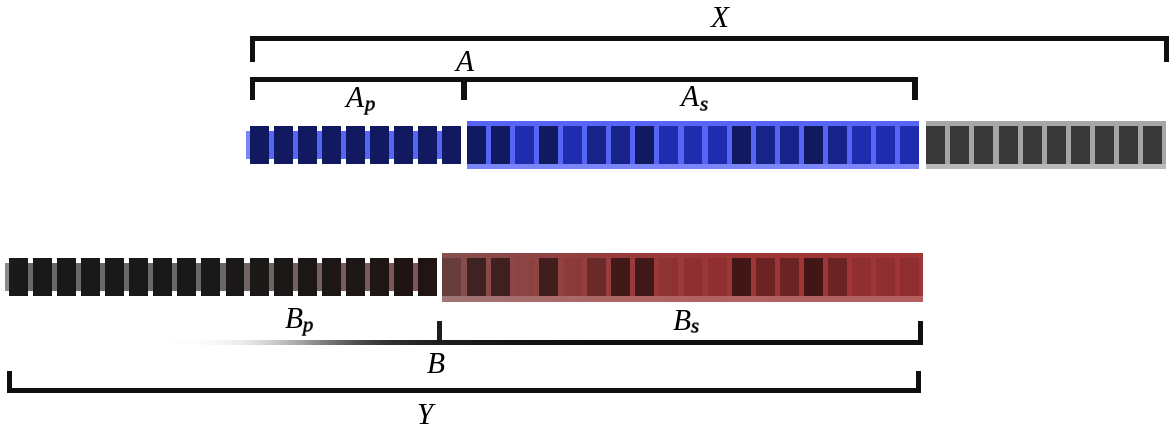
\includegraphics[width=.8\textwidth]{images/blind.png}
\caption[Overlaps between two strings $X$ and $Y$, illustrating the portion of the overlap with an unknown length.]{Some overlap between strings $X$ and $Y$, with overlapping sections $A$ and $B$, each of which is divided into prefixes $A_p$ and $B_p$ respectively and suffixes $A_s$ and $B_s$ respectively. The length of $B_p$ is unknown if the distance between strings is defined in terms of edit distance.}
\label{fig:blind}
\end{figure}

Observe that the known symbol-offset into $X$ of the query string implicitly defines the boundary between $A_p$ and $A_s$; Thus, these substrings have known lengths $|A_p|$ and $|A_s|$. Length $|B_s|$ is also known, as the search process could easily record and manipulate local variables on the stack to keep track of the string \glspl{derivation} associated with each node in the search tree.


In the event of \gls{Hamming distance} being used as the \gls{error distance}, by definition $|A|=|B|$. Therefore, both overlaps comprising $C$ are known, and can be used for the \gls{verification step}. However, using \gls{edit distance} as the distance measure, the same property does not hold. Although $|B_s|$ is indeed known, the same cannot be said for $|B_p|$. Thus, it becomes unclear where to draw the boundary between the suffix $B$ of $Y$ and the rest of $Y$ not involved in the overlap. Of course, possible values for $|B_p|$ are constrained by the length of $Y$; Clearly the overlap length cannot exceed the length of the strings involved. Even better, the $|B_p|$ is obviously related to $|A_p|$, and as the number of indels between $X$ and $Y$ is restricted, the difference in length between these two substrings is also restricted. Still, a candidate with non-specific overlap length(s) cannot be verified.

It would appear then that the only way to cover all solutions is to consider all possible values of $|B|$ within the bounds, and generating a separate candidate for each possibility; Indeed, this approach is quite practical if the \gls{error rate} limit is expected to be low (resulting in a tight bound). Consider a string $X$ with an overlap length of 50 characters, using an error rate limit of 2\%. A naive estimate bounds the length of $Y$'s overlap to the small range of [49, 51]; Any other lengths would necessitate more \glspl{indel} than would be permitted. Knowledge of how many errors are known to exist between $A_s$ and $B_s$ can serve to tighten this bound even further. Continuing our example, just one error between $A_s$ and $B_s$ would imply with certainty that $B_p=50$ for the overlap to have a hope of verifying.

In our \aspop{} solver implementation, exactly this range method is used, potentially generating a handful candidates per \gls{match location} when edit distance is used as the distance measure.
 
Another more robust solution would necessitate a modified \gls{verification step} and candidate representation, where each candidate stores the \textit{range} of lengths for $B$. A well-known dynamic programming algorithm for edit distance could be altered to return distance values for all overlap lengths in this range in tandem. This, however, would necessitate further complicating the implementation and cluttering the system with complex deduplication methods to resolve candidates that contain overlapping overlap ranges.




\subsection{Modified Edit Distance}
Many applications of an \aspop{} solver are interested in the lengths of the prefix and suffix of strings in overlaps; For instance, longer overlap \glspl{solution} are less likely to be \textit{false}, only being facilitated by some `lucky' read \glspl{error}.
 
The standard \gls{edit distance} measure allows for \glspl{insertion} or \glspl{deletion} at either end of an overlap. This runs counter to our understanding of a `real' overlap. With available indel errors to make, the \gls{query} search would indiscriminately retain solutions that are only possible by `padding' the ends of the overlap with inserted symbols to extend the overlap length as much as \bfit{pE} will allow. This might exaggerate the degree to which two strings overlap. To mitigate this, our implementation uses a \textit{modified} edit distance function, wherein the very end symbols of overlaps are prohibited from being the result of insertions or deletions. A byproduct of this decision renders the edit distance between very short strings (such as strings `GGG' and `GG') undefined, with no way to go from one to the other without violating the new rule. In practice, good solutions are required to be substantially longer by the \bfit{t} parameter anyway, so this requirement doesn't cause any solutions to be overlooked.
 
Accepting this modified edit distance allows for increased strictness for the \gls{candidate condition}, reducing the number of generated candidates via redundant search paths. Whenever a search step most recently performed an insertion or deletion, it suppresses candidate generation for one step; Any candidates for solutions thereby overlooked in such a suppressed search node must be reachable with another, and will yield a candidate in that node instead of doing so in both. In this way, the modified edit distance defines the solution set to miss just a few elements, but cuts down a significant number of redundant candidates.







\section{Complexity}
\label{complexity}

\vali{} offer some time and space complexity bounds for a problem of this nature in general and for the \gls{text index} search discussed in Section \ref{P2text_index} \cite{vali2012}. In this section, we attempt to bound the time complexity specifically when using a \gls{suffix filter} algorithm. We also discuss the behavior one can expect from the implementation in terms of space.

\subsection{Time Complexity}
\label{time_complexity}



Often \glspl{filter algorithm} have abysmal worst-case time complexities, but tend to do significantly better in the average case \cite{kuch2014}; This is a consequence of the foundations of their \glspl{filter criterion} relying on assumptions about the problem instance that experience tells us are extremely likely to hold. In our case, actual runtime is sensitive to a host of variables including inherent properties of the input data set itself (as can be seen from the experiments in Section \ref{phase2}).

Key to the runtime of \textit{both} steps of the \gls{suffix filter} algorithm is the shape of the \gls{query} search tree in the \gls{search step}, as this determines the time complexity of this step, but also the number of candidates; Consequentially, this also determines the time spent in the \gls{verification step}. For this reason, we attempt to bound the \textit{number} of nodes in the entire search tree for an arbitrary \gls{query} search, and reason forward from there. This bound is given as:
$$\mathcal{O}(b^2 \cdot{} a^b \cdot{} l^b \cdot{} b!)$$

where\\


% \\[3mm]
\vspace{-2mm}
\hspace{0.6cm}
\begin{tabular}{lcl}
$l $ &:& length of the longest block in the \gls{pattern}\\
$b $ &:& number of pattern blocks i.e. $b=K+1$\\
$a $ &:& \parbox[t]{8.3cm}{number of symbols available for a \gls{mismatch}. i.e. $a=|\sigma{}|-1$ for symbol alphabet $\sigma{}$}
 \end{tabular}
\\[3mm]

To arrive at this expression, we have made the following assumptions:

\begin{itemize}
\item No branch in the search tree is ever \textit{pruned}. Indeed, this is only reasonable in the worst case and should be interpreted as such. Realistically, branches being regularly pruned is the assumption that the entire \gls{filter algorithm} relies on to offer an advantage. Unfortunately, for arbitrary \glspl{text}, we can make no such assumption.
\item The algorithm uses the simplest of \glspl{filtering scheme} (that of \kark{}) with only one redundant block per pattern prefix so lemma \ref{lemma1} is satisfied minimally.
\item Blocks are of equal lengths. Indeed this is very unrealistic, but this is the effect of using this bound. In reality, some blocks are shorter than the defined $b$. This fact makes our upper bound more \textit{conservative} than is strictly necessary. However, assuming the basic \vali{} \gls{partitioning scheme} this assumption holds for all blocks but one; All blocks have some \bfit{p} length, except the last which has some length $x$ in $1\leq{}x\leq{}\bfit{p}$.
\end{itemize}

Understanding this bound and how it was composed is best-done by breaking it down and enlisting the help of two smaller subproblems:

\begin{enumerate}
\item \textbf{Number of nodes in a 1-block long tree with $\bfit{pE}=m$}

The search performed by the \gls{text index} is structured as a branching tree of string \glspl{derivation}, with nodes for each derived prefix of the query (and thus, substring of the pattern). Each node (and each symbol) involved falls into a particular pattern \gls{block}. The total number of nodes in the search tree is what we are after, but this term can be further decomposed into the number of nodes \textit{within} a certain block.

Consider the first block with $\bfit{pE}=0$. The search path can do nothing but linearly walk the block to the end, requiring $l$ such steps. Thus, this block contains $l$ nodes.

For a tree in a block given $\bfit{pE}=1$, the search steps through $l$ symbols in the block's string, at each step producing $|\sigma{}|=a+1$ branches in total (with $a$ branches for an error-introduction steps + 1 step for matching the query symbol). The resulting child-branches of error steps have $\bfit{pE}=0$ and thus can do no more than to walk to the end of the block much as the first $\bfit{pE}=0$ block did. The number of nodes in this subtree is $l+a\cdot{}((l-1)+(l-2)+...+1)$, as each linear subtree from each error has a shorter distance to go the later it forks off from the 0-error path.

Lastly consider the case of a search beginning in a block with $\bfit{pE}=2$.  Along with the usual single 0-error linear walk to the end, each symbol position can introduce an error and bring rise to the $\bfit{pE}=1$ block problem described above, but with a `shorter block', so to speak. This manifests itself as a 2-dimensional summation series:
$$l + a\cdot{} (a((l-1)+(l-2)+...+1) + a((l-2)+(l-3)+...+1) +...+ 1 )$$
With each increase in \bfit{pE}, the dimension of this series is incremented; Conceptually, each increase instantiates $a\cdot{}l$ instances of the subproblem with one less \bfit{pE} and a `new block length' of however many symbols lie between the current index and the end of the block. Even the base case of $\bfit{pE}=0$ can be written as $l + a\cdot{}(0+0+...+0)$. In this fashion, the number of nodes in such a 1-block-long tree for arbitrary $\bfit{pE}=m$ is in the order of: $$\mathcal{O}(a^m \cdot{} l^m)$$




\item \textbf{Number of leaves in a tree ending after the $n$th block having spent $m$ errors so far}

We are also interested in how many \textit{leaf nodes} exist at the end-boundary of a given block, and how many errors those nodes have spent so far; These nodes will be roots of subtrees in the subsequent block.

Consider the base case of a tree for a block with $\bfit{pE}=0$. As before, all that the search can do is walk forward, with no branching whatsoever, so this tree ends up reaching the end of its block with just one 0-error leaf.

Next, consider a tree comprised of two blocks. As before, the unique path without any error-branching is always an option, and will produce a single 0-error leaf at the end of the 1st block, as well as the 2nd block. Once beyond the first block, the search can recursively consider positions to spend its stored \bfit{pE}, each time introducing an error in $a$ unique ways. This is possible in every index of the second block; Each resulting child branch will have no more \bfit{pE} to spend, forcing it to simply match the remaining query symbols linearly. In total, this tree will have $l \cdot{} a$ such 1-error branches.

For one last step, consider adding a third block. This tree has the single ever-present 0-error node at the end of the 2nd block. Any 1-error paths could only have forked from the 0-error path in the second or third blocks, resulting in $2 \cdot{} l \cdot{} a$ 1-error leaves. As errors are introduced sequentially, it can be reasoned that any 2-error path at some point forked off a 1-error path. This fork could have occurred at any index using any of $a$ symbols, but entirely \textit{after} the second block, as prior to this there is insufficient \bfit{pE} to introduce the second error. As such, there will be $2 \cdot{} l \cdot{} a$ such 2-error leaves.

The same reasoning allows us to enumerate the kinds of leaves for some $m$th block. Assuming that the maximal number of errors is smaller than $l$ (a reasonable assumption), the branching can occur at any index in blocks where \bfit{pE} is high enough to facilitate the introduction of the error. As such, the number of $m$-error leaves at the end of an $n$-long \gls{block sequence} search is given by:
$$\prod_{i=1}^{m} l \cdot{} a \cdot{} (n-i)$$
which is in the order:
$$\mathcal{O}(\dfrac{l^m \cdot{} a^m \cdot{} n!}{(n-m-1)!})$$



\end{enumerate}

The computation of the number of nodes in a query search \textit{within} some block $B$ can be done with use of subproblems 1 and 2. The total nodes within this block can be partitioned into various \textit{subtrees}, according to their value of \bfit{pE} at the root. Subproblem 1 allows us to compute the number of nodes within each such tree, and subproblem 2 allows us to compute how many such trees exist within the block (by considering which leaves are exposed at the end of the \textit{prior} block). As such, the number of nodes in the $(n+1)$th layer of such a search tree can be given as:
$$\sum_{m=0}^{n-1} \dfrac{l^m \cdot{} a^m \cdot{} n! }{(n-m-1)!} \cdot{a^{(n-m)} \cdot{} l^{(n-m)}}$$

which can be simplified to:
$$\sum_{m=0}^{n-1} \dfrac{l^n \cdot{} a^n \cdot{} n! }{(n-m-1)!}$$


Finally, the sum of all nodes in the entire query search is the number of nodes in a block (given above), summed across all of the blocks in the pattern comprised of $b$ blocks\footnote{For brevity in the formula, the inner summation defines the nodes in block $N+1$ and not $N$. Therefore, this outer summation iterates over values 0 to $b-1$, but is logically iterating over each block from the 1st to the $b$th.}:
$$\sum_{n=0}^{b-1}\sum_{m=0}^{n-1} \dfrac{l^n \cdot{} a^n \cdot{} n! }{(n-m-1)!}$$

If one were really pressed to extrapolate a worst-case time complexity for the algorithm from the information provided thus-far, one could come up with the bound\footnote{Each node in the search tree relies on the result of a `rank' call of the \gls{text index} to find the next `occurrence range' (corresponding with thinning out the \gls{match location} set). The complexity of this call would multiply the complexity; However, in most cases the cost of this call is a large constant value by making use of `checkpoints', and thus the multiplicative factor doesn't change the time complexity.} of:
\begin{gather*}
\mathcal{O}((b^2 \cdot{} a^b \cdot{} l^b \cdot{} b!) \cdot{r} \cdot{} b \cdot{} c \cdot{l})\\
 = \mathcal{O}(b^3 \cdot{} a^b \cdot{} l^{b+1} \cdot{} b! \cdot{r} \cdot{} c)
\end{gather*}

where $r$ represents the number of \glspl{read} in the data set and $c$ represents the upper bound for the number of \glspl{candidate}\footnote{We assume that there is no concept of candidate deduplication at all. This is of course unrealistic in any reasonable implementation.} generated at search step (i.e. each node of the tree). An \textit{egregiously} conservative bound would set $c$ to the length of the text, considering that a candidate might be generated at every available index in the text. More reasonably, one could instead set $c=r$, which makes the assumption that no search step will generate numerous candidates per read (not strictly true but likely more representative of the truth). The remaining new terms $b$ and $l$ correspond, respectively, with the number of query searches per \gls{pattern} and the worst-case cost of computing \gls{Hamming distance} per candidate.

Section \ref{aux:nodes} explores the proportion of pruned nodes in query search trees in a more \textit{practical} sense. This is intended to demonstrate the difference in complexity between the worst-case execution and that of a realistic case.



\subsection{Space Complexity}
\label{space_complexity}

These \gls{suffix filter} algorithms are quite unique in that the worst-case space complexity is significantly less interesting to a user than knowledge of the number of worker threads for an execution. Space taken is strongly related to the shape of the search tree and the number of \glspl{candidate}, both  of which are described in Section \ref{time_complexity} above.

The execution of the \aspop{} solver spawns a number of worker threads, each drawing from a pool of \glspl{task}, corresponding to a pool of \glspl{read} to treat as the \gls{pattern} in turn (See Section \ref{solving_ASPOP} for details). Threads have a shared resource, namely the \gls{text index} and its associated \gls{text}. Aside from this constant space (which is approximately $l \cdot{} r$), space consumption scales linearly with the number of simultaneous working threads. 

Space taken by a thread changes throughout the execution, ascending from nothing to a peak between the \gls{search step} and the \gls{verification step}, then decreasing down to just the space required to store the thread-local \gls{solution} set\footnote{The implemented \aspop{} solver also has an optional parameter to enable `greedy output'. This results in tasks printing solutions to file at the end of the task instead of retaining them. This can save space when many solutions are expected, but removes some guarantees for the uniqueness and order of solutions in the output file.} associated with the task's pattern. During the search step, a \textit{depth-first-search} is initialized once per filter, creating a recursive tree of steps over a substring of the pattern (the \gls{query} string). The size and space on the stack taken by this tree is hard to predict, as in most cases branches are frequently\footnote{See Section \ref{aux:nodes} for an experiment that seeks to estimate \textit{how} frequently search nodes are pruned in the average case.} pruned. What is certain, however, is that throughout this search process, the size of the \gls{candidate} set is \textit{nondecreasing}. After the search is complete, the tree no longer takes up space, and the \gls{solution} set is populated (but at the same time, the candidate set is emptied). Thus, the space taken up by a \gls{task} in the verification step is \textit{nonincreasing}\footnote{This doesn't consider some stack-frames needed to compute whether a single candidate verifies.}. The space taken up at the end of a task is only back down to nothing if no solutions were found by this task, as solutions are aggregated for sorting.

In phase 3 of the experiments, given in Section \ref{phase3}, the space behavior of the \aspop{} solver is seen in action.